\documentclass[12pt,final,slidescentered,usepdftitle=true]{beamer}
% "final" and "draft" are optional to increase the speed of compilation
% "slidescentered", "slidestop" are options
% override these options for individual slides with "t", "c" or "b"
% "handout" is another class option overriding all overlays

        %Included for Gather Purpose only:
        %input "../../literature.bib"
%%%%%%%%%%%%%%%%%%%%%%%%%%%%%%%%%%%%%%
% Setting up the presentation layout %
%%%%%%%%%%%%%%%%%%%%%%%%%%%%%%%%%%%%%%

% To exclude the backup slides from being included in the ``totalframenumber'' count:
\makeatletter
\let\appendixtotalframenumber\empty
\def\mainend{-1}
\let\appendixorig\appendix

\def\appendix{
  \edef\mainend{\theframenumber}
  \immediate\write\@auxout{\string\global\string\@namedef{mainendframenumber}{\mainend}}
  \appendixorig
  \def\inserttotalframenumber{\appendixtotalframenumber}%
  \setcounter{framenumber}{0}
}

\def\newblock{\hskip .11em plus .33em minus .07em}

\def\pageatend{
  \edef\appendixend{\theframenumber}
  \ifnum\mainend>0%
  \immediate\write\@auxout{\string\global\string\@namedef{appendixtotalframenumber}{\appendixend}}%
  \immediate\write\@auxout{\string\global\string\@namedef{inserttotalframenumber}{\mainend}}%
  \immediate\write\@auxout{\string\@writefile{nav}{\noexpand \headcommand {%
        \noexpand \def\noexpand \inserttotalframenumber{\mainend}}}}%
  \immediate\write\@auxout{\string\@writefile{nav}{\noexpand \headcommand {%
        \noexpand \def\noexpand \appendixtotalframenumber{\appendixend}}}}%
  \else
  \fi
}
\AtEndDocument{\pageatend}
\makeatother

% Defining colours used in the document:
\usepackage{color}
\definecolor{HUBlue}{cmyk}{1,.6,0,.2}
\definecolor{HURed}{cmyk}{0,.9,.8,.4}
\definecolor{HUGreen}{cmyk}{.9,.1,.8,.4}
\definecolor{HUSand}{cmyk}{0,.05,.5,.2}
\definecolor{HUGrayGreen}{cmyk}{0,0,.1,.2}
\definecolor{HUBlueGray}{cmyk}{.1,0,0,.2}
\definecolor{darkblue}{rgb}{0,0,0.55}
\definecolor{brightgreyblue}{rgb}{0.92,0.92,0.94}
\definecolor{darkred}{rgb}{0.8,0.00,0.00}
%\setbeamercolor{alerted text}{fg=darkred}
\usepackage{pgf,pgfarrows,pgfnodes,pgfautomata,pgfheaps}


\usecolortheme[named=HUBlue]{structure}
\usecolortheme{sidebartab}
\setbeamercolor{alerted text}{fg=HURed}
% Generating the grey foot line:
%\setbeamercolor{footlinecolor}{fg=HUBlue}
\setbeamercolor{footlinecolor}{fg=HUBlue,bg=HUGrayGreen!50}
\setbeamertemplate{footline}
  {\begin{beamercolorbox}{footlinecolor}
     \vskip3.5pt
     \insertsectionnavigationhorizontal{0.85\paperwidth}{}{}%
     \vspace{-0.9\baselineskip} \hfill \normalfont \insertframenumber\,/\,\inserttotalframenumber%
     \hspace{8pt}
     \vskip4pt
   \end{beamercolorbox}
  }
 \setbeamertemplate{caption}[numbered]
\setbeamertemplate{caption}{\small\textbf{\usebeamercolor[fg]{structure}\insertcaptionname~\insertcaptionnumber.} \insertcaption}

% Turning off the navigation symbols on the bottom of the frames:
\beamertemplatenavigationsymbolsempty
\beamertemplatetransparentcovered
% alternatively: \beamertemplatetransparentcovereddynamic

\usepackage{amsmath,amssymb}
\usepackage{pgf,pgfarrows,pgfnodes,pgfautomata,pgfheaps}
\usepackage{stackengine}

% Choosing a font combination (serif, non-serif and mono-spaced font):
% \usepackage[sc]{mathpazo} \usepackage[scaled=0.9]{helvet} \usepackage{courier}
% Alternative font combinations:
% \usepackage{fourier} \usepackage[scaled=0.84]{berasans} \usepackage[scaled=0.84]{beramono}
% \usepackage{mathptmx} \usepackage[scaled=0.9]{helvet} \usepackage{courier}
\usepackage[charter]{mathdesign} \usepackage{berasans} \usepackage{beramono}
% \usefonttheme[stillsansseriflarge]{serif}
\usefonttheme{serif}
\usefonttheme{structurebold}

\frenchspacing  % prevents the enlarged whitespace after a dot
\sloppy

% The following command has the effect that at the beginning of each section, the outline
% slide is repeated, with the current section being highlighted:
\AtBeginSection[]
  {\begin{frame}<beamer>
     \frametitle{~}
     \tableofcontents[currentsection]
   \end{frame}
  }

% Enable hyphenation on Beamer slides:
\usepackage{ragged2e}
\let \raggedright \RaggedRight
\sloppy
\hyphenpenalty=500
\setbeamersize{text margin right=25pt}

%% Edit Holger:
%\setbeamertemplate{footline}
%  {\vskip-7.5pt\hspace{7pt}
%   % \textcolor{black}
%   {\usebeamercolor[fg]{navigation symbols}\fontseries{m}\selectfont\insertframenumber\,/\,\inserttotalframenumber}
%   \vskip4pt
%  }

% The following package enables so-called hanging punctuation.
% That is, when a punctuation sign like ":", ".", "-" etc.
% is found at the beginning or end of a line, it is protruded a little into the page margin.
% This leads to so-called "optical margin alignment," because the protrusion
% makes the margin alignment look straighter.
\usepackage[protrusion=true, expansion=false, kerning=true]{microtype}
\SetExtraKerning[unit=space]
  {encoding={*}, family={*}, series={*}, size={*, footnote size}}
  {\textemdash={325,325}}

% If you use BibTeX:
\usepackage[authoryear,semicolon]{natbib}

\makeatletter

\DeclareRobustCommand\citepos
  {\begingroup\def\NAT@nmfmt##1{{\NAT@up##1's}}%
   \NAT@swafalse\let\NAT@ctype\z@\NAT@partrue
   \@ifstar{\NAT@fulltrue\NAT@citetp}{\NAT@fullfalse\NAT@citetp}}

\makeatother


%%%%%%%%%%%%%%%%%%%%%%%%%%%%%%%%%%%%%%%%%%%%
% Loading additional useful LaTeX packages %
%%%%%%%%%%%%%%%%%%%%%%%%%%%%%%%%%%%%%%%%%%%%

\usepackage[latin1]{inputenc}  % enables you to input "Umlaute" as 'ä' instead of '\"a' etc.
\usepackage{graphicx}


% \usepackage[pdftex, pdftitle={Insert title of the talk/lecture},
%   pdfauthor={You 1 and You 2}, pdfsubject={Insert subject of the talk/lecture},
%   bookmarks=true, bookmarksopen=true, bookmarksnumbered=true, bookmarksopenlevel=2, colorlinks=true,
%   pdfpagemode=UseOutlines, pdfview=Fit, pdfstartview=Fit, pdffitwindow=false, linkcolor=darkblue,
%   citecolor=darkblue, urlcolor=darkblue]{hyperref}
\hypersetup{colorlinks=true, linkcolor=HUBlue, citecolor=HUBlue, urlcolor=HUBlue}
\urlstyle{same}

\usepackage{verbatim}
\usepackage{listings}
% \usepackage[activate]{pdfcprot}

\usepackage{ulem}
%\usepackage{subeqn}
\usepackage{mathrsfs} % this is for Vetter's differentation operator
\usepackage{rotating}
\usepackage{verbatim}
\usepackage{multirow}
\usepackage{multicol}
\usepackage{afterpage}
%\usepackage{footmisc}
\usepackage[justification=centering]{caption}
\usepackage{arydshln} % for dashed lines in arrays
\usepackage{hyperref}
\newtheorem{assumption}[theorem]{Assumption}
\newtheorem{proposition}[theorem]{Proposition}

\usepackage{epstopdf}
%%%%%%%%%%%%%%%%%%%%%%%%%%
% Some new math commands %
%%%%%%%%%%%%%%%%%%%%%%%%%%

\newcommand{\rdmatrix}[1]{\left(\,\begin{matrix}#1\end{matrix}\,\right)}
\newcommand{\sqmatrix}[1]{\left[\,\begin{matrix}#1\end{matrix}\,\right]}
\newcommand{\E}{\mathrm{E}}
\newcommand{\Var}{\mathrm{Var}}
\newcommand{\Cov}{\mathrm{Cov}}
\newcommand{\dd}{\mathrm{d}}
\newcommand{\scL}{\mathcal{L}}

\makeatletter
\renewenvironment{subarray}[2][c]{%
  \if#1c\vcenter\else\vbox\fi\bgroup
  \Let@ \restore@math@cr \default@tag
  \baselineskip\fontdimen10 \scriptfont\tw@
  \advance\baselineskip\fontdimen12 \scriptfont\tw@
  \lineskip\thr@@\fontdimen8 \scriptfont\thr@@
  \lineskiplimit\lineskip
  \ialign\bgroup
    $\m@th\scriptscriptstyle##$\hfil\crcr
}{%
  \crcr\egroup\egroup
}
\makeatother
\renewcommand{\substack}[2][c]{\subarray[#1]{c}#2\endsubarray}
%%%%%%%%%%%%%%%%%%%%%%%%%%%%%%%%%%%%%%%%%%%
% The information shown on the title page %
%%%%%%%%%%%%%%%%%%%%%%%%%%%%%%%%%%%%%%%%%%%

\title[\fontseries{rm}\selectfont whateverwecallit]
      {\\ QuantNet 2.0 @ GitHub}
 \subtitle{ }
%Generalized Exogenous Processes in DSGE:\\ A Bayesian Approach
%Bayesian Estimation of Autoregressive Moving-Average Processes as Exogenous Shock Processes in DSGE Models
% \author[]{\href{mailto:jim.beamer@wiwi.hu-berlin.de}{Jim Beamer}}
\author[Borke, Neuhoff]{Lukas Borke and Daniel Neuhoff}
\institute{\small  Humboldt-Universit\"at zu Berlin \hspace{2em} CRC 649}
% Remark: It's Humboldt University's official policy that the name "Humboldt-Universität zu Berlin"
% is NOT translated to foreign languages.
\date{\small November 2015}  % or provide fixed date
\pgfdeclareimage[height=2cm]{hu-logo}{../figs/hu_logo}
\pgfdeclareimage[interpolate=true,height=1.15cm]{sfb-logo}{../figs/SFB649_Text}
%\pgfdeclareimage[height=0.95cm]{UBo-logo}{Images/Logo-UBo-h24-RGB}
% \titlegraphic{\vspace{0.25cm}\pgfuseimage{hu-logo}}
% \titlegraphic{\vspace{0.1cm} \pgfuseimage{hu-logo} \hspace{1.5cm} \raisebox{10pt}{\pgfuseimage{sfb-logo}}}
% \titlegraphic{\vspace{0.25cm}\pgfuseimage{UBo-logo}}


\AtBeginDocument{%
  \pgfdeclareverticalshading{beamer@headfade}{\paperwidth}
  {%
    color(0cm)=(HUGrayGreen!50);
    color(1cm)=(HUGrayGreen!50)%
%    color(0cm)=(bg);
%    color(1cm)=(bg)%
  }
}

\addtoheadtemplate{\pgfuseshading{beamer@headfade}\vskip-1cm}{}
\AtBeginDocument{%
  \pgfdeclareverticalshading{beamer@footfade}{\paperwidth}
  {%
    color(0cm)=(HUGrayGreen!50);
    color(0.5cm)=(HUGrayGreen!50)%
  }
}

\addtoheadtemplate{\pgfuseshading{beamer@footfade}\vskip - \paperheight}{}

\let\Tiny=\tiny
%%%%%%%%%%%%%%%%%%%%%%%%%%%%%%%
% Now the actual text begins: %
%%%%%%%%%%%%%%%%%%%%%%%%%%%%%%%

\usepackage{hyperref}
\hypersetup{pdfpagemode=FullScreen}

\begin{document}
\setlength{\baselineskip}{2.9ex}

{\setbeamertemplate{footline}{}\frame{\titlepage}}
\addtocounter{framenumber}{-1}

\frame{
  \frametitle{Outline}
  \tableofcontents
  }

\section[RJMCMC]{Reversible Jump Markov Chain Monte Carlo}
\frame{
	\frametitle{Reversible Jump MCMC}
	Standard practice for approximation of posterior distributions for model parameters: Metropolis-Hastings samplers \vspace{0.5em}
	
	\textbf{Problem:} Want to analyze posterior distribution also spanning model space \\ 
	\indent $\Rightarrow$ Dimensionality of parameter space varies\\
	\vspace{0.5em}
		
	\textbf{Solution:} Reversible Jump Markov Chain Monte Carlo
	\begin{itemize}
		\item Generalization of Metropolis-Hastings samplers
		\item Samples from a joint posterior distribution across different models and their corresponding parameter spaces
	\end{itemize}	
}


\frame{
	\frametitle{Posterior Distribution Across Models}
	Posterior distribution across ARMA(p,q) models:
	\begin{center}
		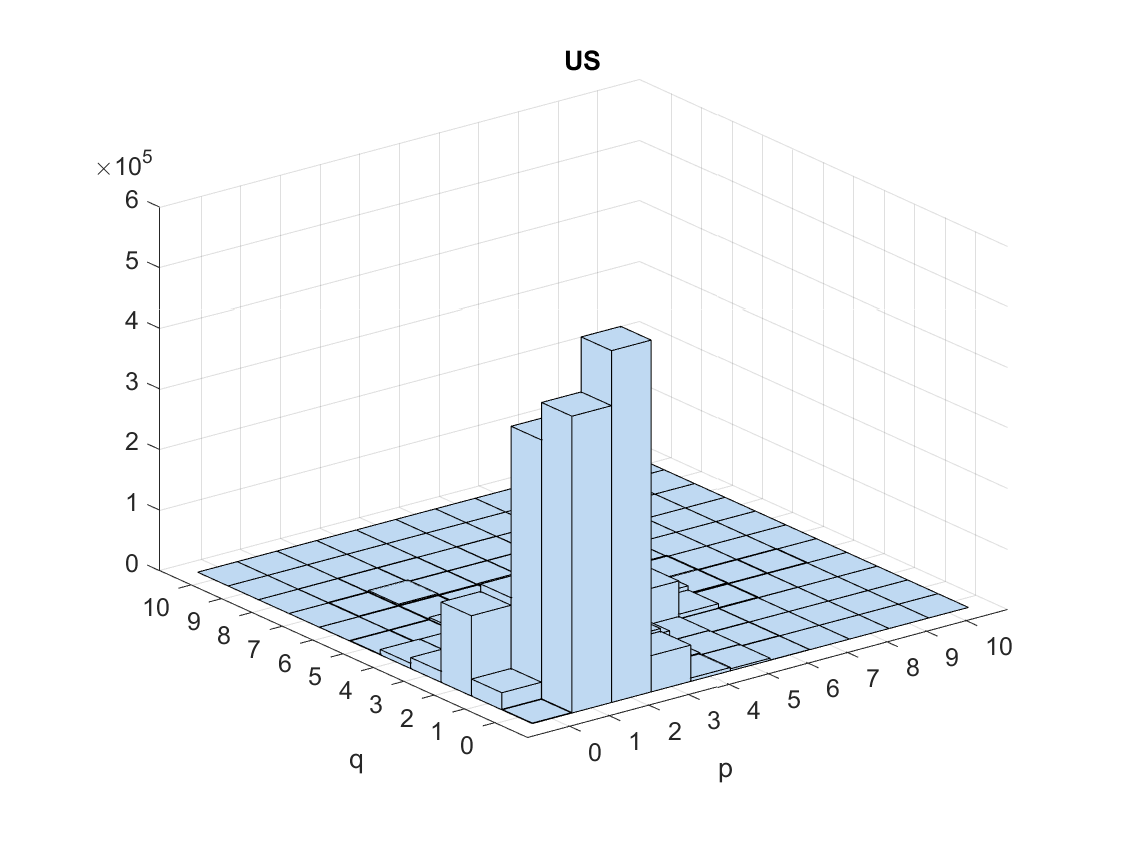
\includegraphics[height=0.6\textheight]{PosteriorPQ_US_Draws_4000000_Filter_FDIFF}
	\end{center}
	$\Rightarrow$ Posterior model probabilities
}

\frame{
	\frametitle{Posterior Distribution: Impulse Responses}
	Can analyze posterior distribution for any statistic while accounting for model uncertainty!
	\begin{center}
		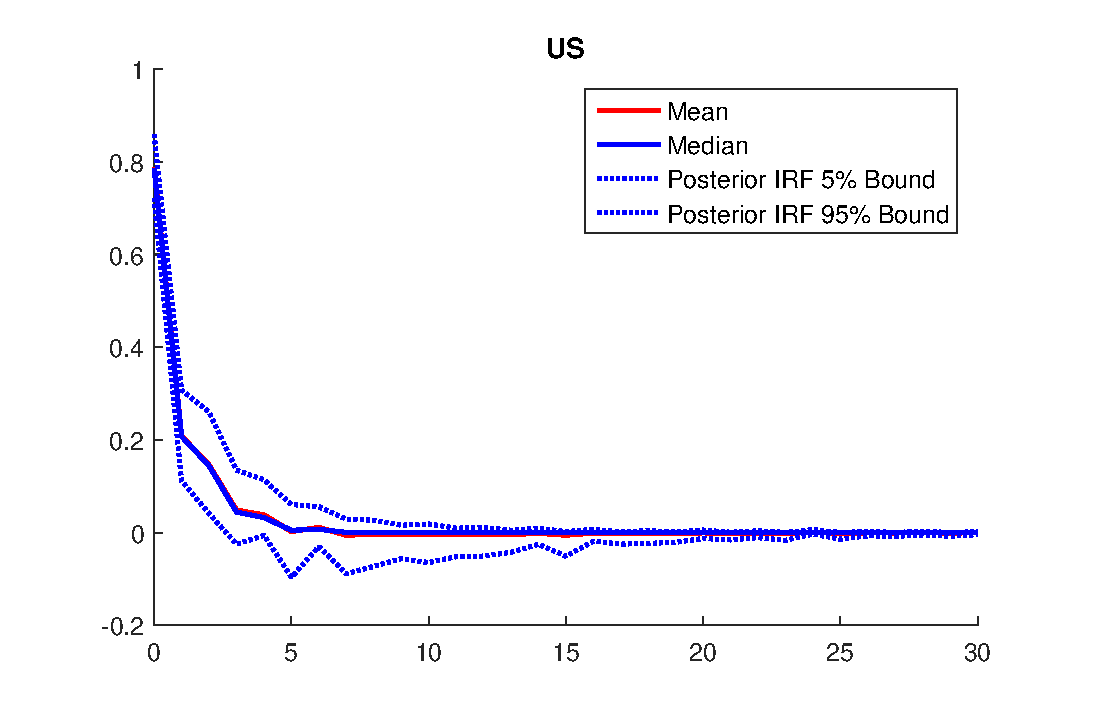
\includegraphics[height=0.6\textheight]{IRFs_Scaled_US_FDIFF}
	\end{center}
	
}

\section[Modern Science]{Modern Scientific Practice}

\frame{
	\frametitle{Modern Scientific Practice}
	Modern scientific practice:
	\begin{itemize}
		\item Transparency
		\item Reproducibility
	\end{itemize}
	Also: Want to publicize new technologies! \\ \vspace{0.5em}
	\textbf{Problem:} Need and want to publish our technologies and data!
}


\section{GitHub and QuantNet 2.0}

\frame{
	\frametitle{The Solution}
		\begin{center}
			{\Large 		\textbf{QuantNet 2.0}}

				\vspace{0.5em}

				
\includegraphics[height=0.6\textheight]{qletlogo}
				% 2 blanks between pictures
				\ \
				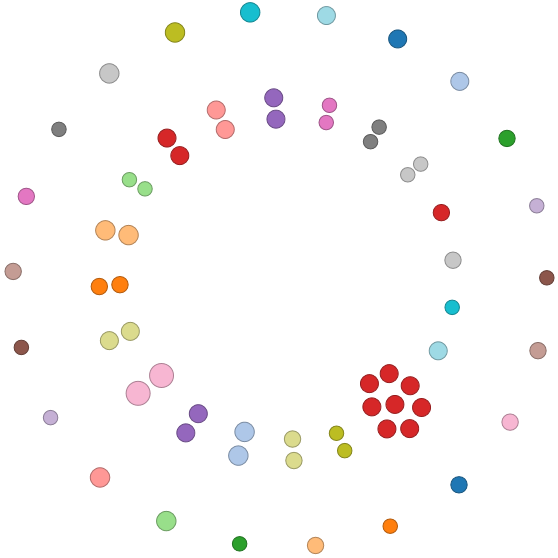
\includegraphics[height=0.6\textheight]{QN2}

		\end{center}
}

\frame{
	\frametitle{The Solution}
	\textbf{QuantNet 2.0 -  The Next Generation}
	\begin{itemize}
		\item $\approx$ 2000 Quantlets
		\item Technology to easily share data and programs
		\item Searchable technology
		\item Enabled collaboration via seamless GitHub integration
		\item Connections between technologies
	\end{itemize} \vspace{0.2em}
	\textbf{Boosting transparent and reproducible science}

}

\section{GitHub}
  
\frame{
	\frametitle{What is GitHub?}		
		
	\begin{center}
		
\includegraphics[scale=0.25]{githublogo2}
	\end{center}
	%\vspace{0.5em}	

		\begin{itemize}
			\item {\hfil A distributed version control system (Git) }
			\item {\hfil A collaboration platform (Hub) }
		\end{itemize}

	\begin{center}
		
\includegraphics[scale=0.33]{github-social-coding_crop}
	\end{center}

		
}
%
%\frame{
%	\frametitle{Why use GitHub?}
%	\begin{itemize}
%		\item Version control
%		\item Distributed development
%		\item Easy branching and merging
%		\item Integration with many IDEs
%		\item Issue management
%	\end{itemize}
%}
%
%\section{Terminology and Workflow}
%
%\frame{
%	\frametitle{Create GitHub Account}
%	Go to www.github.com to create an account	
%	\begin{center}
%		
\includegraphics[width=0.8\textwidth]{githubsignup}
%	\end{center}
%}
%
%\frame{
%	\frametitle{Install GitHub Application}
%	From www.github.com download and install the desktop application:
%	\begin{center}
%		
\includegraphics[width=0.8\textwidth]{downloadgithubdesktop}
%	\end{center}
%}
%
%
%\subsection{Accessing GitHub}
%
%\frame{
%	\frametitle{GitHub Desktop App}
%	\begin{center}
%		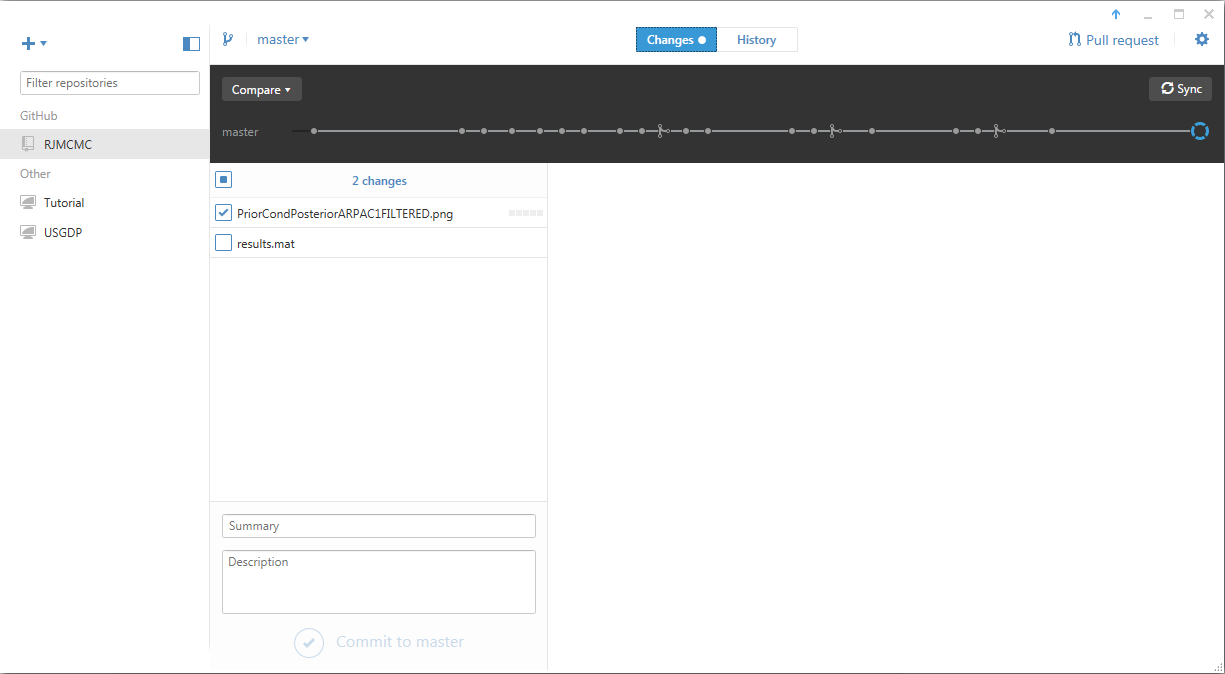
\includegraphics[height=0.6\textheight]{githubdesktop}
%	\end{center}
%}
%
%\frame{
%	\frametitle{Web Interface}
%	\begin{center}
%		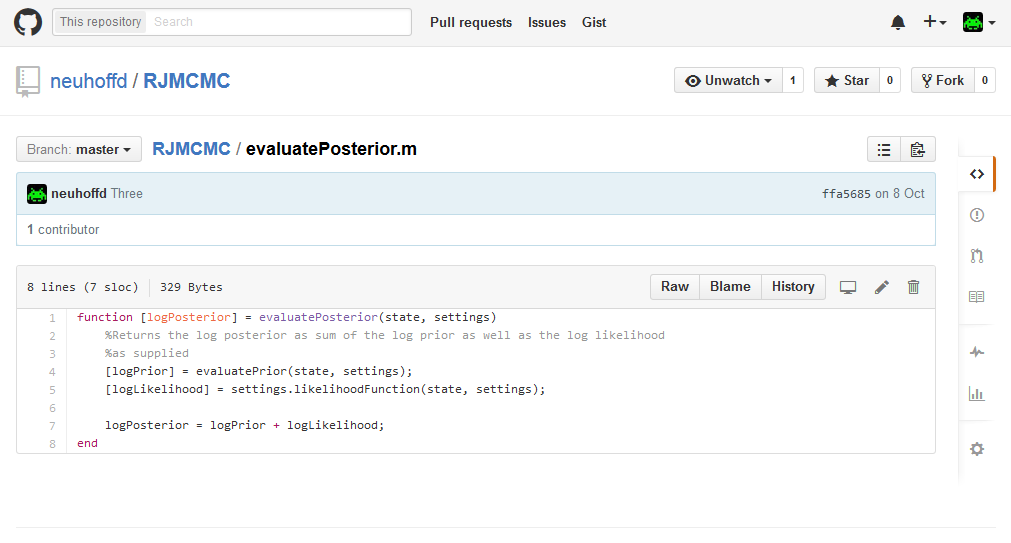
\includegraphics[height=0.6\textheight]{webinterface}
%	\end{center}	
%	
%}
%
%\frame{
%	\frametitle{Command Line}
%	\begin{center}
%		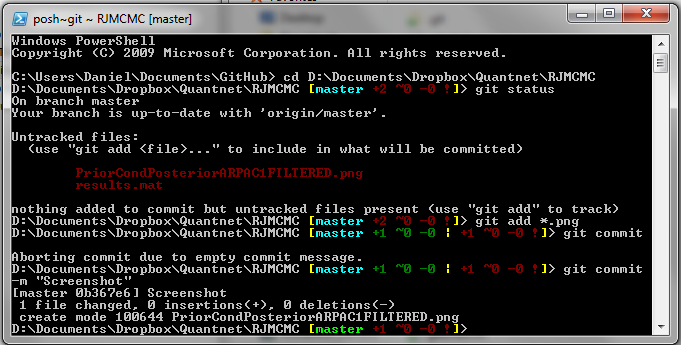
\includegraphics[height=0.6\textheight]{commandline}
%	\end{center}		
%}
%
%\frame{
%	\frametitle{Create Repository}
%	\begin{itemize}
%		\item Most basic element of GitHub
%		\item A project folder containing \textit{all} project files
%		\item Also contains a revision history for each file
%		\item Contains an issue tracker
%	\end{itemize}
%	Three ways to create a repository:
%	\begin{enumerate}
%		\item Desktop app (recommended)
%		\item Web interface
%		\item Command line (advanced)
%	\end{enumerate}
%}
%
%\frame{
%	\frametitle{Develop}
%	Develop your project using GitHub features where sensible:
%	\begin{itemize}
%		\item Manage issues
%		\item Branch/fork code
%		\item Commit changes
%		\item Use pull requests
%	\end{itemize}
%	Keep the style guide in mind!
%}
%
%
%\frame{
%	\frametitle{Manage Issues}
%	Use GitHub issues to record and discuss
%	\begin{itemize}
%		\item Ideas
%		\item Bugs
%		\item Enhancements
%		\item Tasks
%	\end{itemize}
%	You get a searchable history of your discussions! \\ \vspace{0.5em}
%	You can neatly organize any discussion with issue classes
%}
%
%
%\frame{
%	\frametitle{Branch Code}
%	Branching allows you to
%	\begin{itemize}
%		\item work on a copy of the master branch
%		\item to make changes without affecting the whole of the code base
%	\end{itemize}
%	
%}
%
%\frame{
%	\frametitle{Commit Changes}
%	A commit
%	\begin{itemize}
%		\item essentially uploads new versions of files
%		\item is tracked, so you have a history of changes available
%		\item can be rolled back
%	\end{itemize}
%}
%
%\frame{
%	\frametitle{Issue Pull Request}
%	A pull request
%	\begin{itemize}
%		\item asks your collaborators to consider your changes for integration into the master branch (merge)
%		\item can be issued at any time, also for example to share screenshots
%		\item can be augmented by a pull request message to ask for help or @mention other contributors in order to induce them to comment
%		\item initiate a discussion of the changes you made
%	\end{itemize}
%}
%
%\frame{
%	\frametitle{Merge Branches}
%	A merge
%	\begin{itemize}
%		\item integrates your code into the master branch
%		\item preserves a history of your changes by keeping the pull requests (searchable)
%	\end{itemize}
%	
%}
%
%\frame{
%	\frametitle{Finishing up}
%	\begin{itemize}
%		\item Create Metainfo.txt containing information about your Quantlet
%		\item Create readme.md as user guide (good practice)
%		\item Check your code against style guide (somewhat automated for R code)
%		\item Inform QuantNet team
%	\end{itemize}
%}

\frame{
	\frametitle{Advantages of QuantNet 2.0}
	\begin{itemize}	
		\item Fully integrated with GitHub
		\item Proprietary GitHub-R-API developed from core package (Arizona State University)
		\item Ease of discovery and use of your technology
		\item Audit of your technology
	\end{itemize}	

}

\section{Demonstration}


\frame{
	\frametitle{What I did}
	\begin{enumerate}
		\item \textbf{Start:} Create
				\href{https://github.com/neuhoffd/RJMCMC}{GitHub repository}
				with own code
		\item \textbf{Develop:} Develop according to 
				\href{https://github.com/QuantLet/Styleguide-and-Validation-procedure/blob/master/README.md}{style guide}
		\item \textbf{Publish:} Audit and 
				\href{https://github.com/QuantLet}{publish}
	\end{enumerate}		
	\textbf{Your Technology:} Easily \href{http://sfb649.wiwi.hu-berlin.de/fedc/discussionPapers.php}{found}, used, and improved!	
}


%%%%%%%%%%%%%%%%%%%%%%%%%%%%%%%%%%%%%%%%%%%%%%%%%%%%%%%%%%%%%%%%%%%%%%%%%%%%%%%%%%%%%%%%%%%%%%%%%%%%%%%%%%%%%%%%%%%%%%%%
\frame{
	\frametitle{Interactive D3 Visualization}

\begin{figure}[htb]
	\begin{center}
		\href{http://quantnet.wiwi.hu-berlin.de/d3/ia/}{
			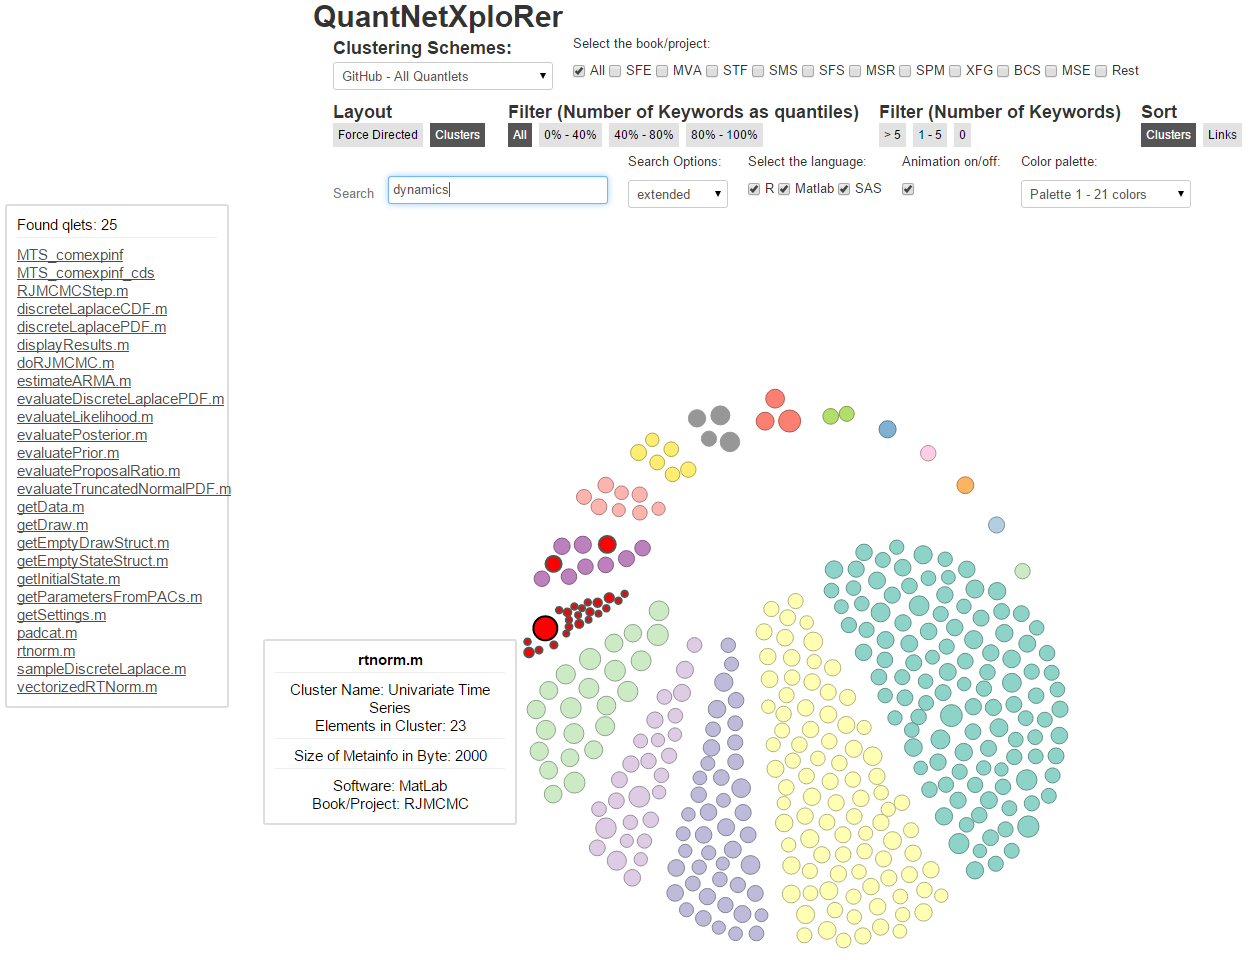
\includegraphics[scale=0.2]{d3_visu_RJMCMC}
		}
	\vspace{-0.25cm}
	\caption{All Quantlets from GitHub in QuantNetXploRer, search term ``dynamics``}
	\end{center}
\end{figure}
}


%%%%%%%%%%%%%%%%%%%%%%%%%%%%%%%%%%%%%%%%%%%%%%%%%%%%%%%%%%%%%%%%%%%%%%%%%%%%%%%%%%%%%%%%%%%%%%%%%%%%%%%%%%%%%%%%%%%%%%%%
\frame{
	\frametitle{Collaboration Timeline via GitHub-API}
		\begin{figure}[htb]
		\begin{center}
				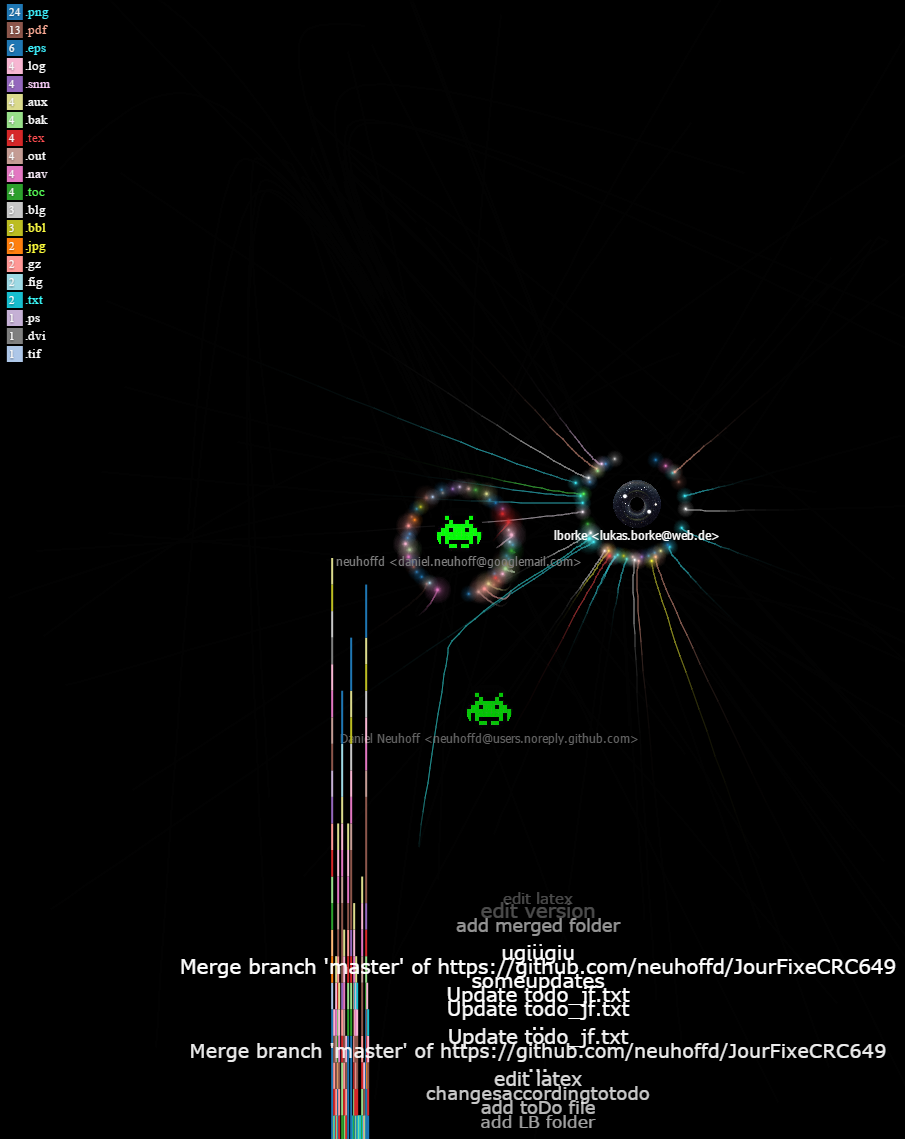
\includegraphics[scale=0.16]{colla_visu1}
				% 2 blanks between pictures
				\ \
				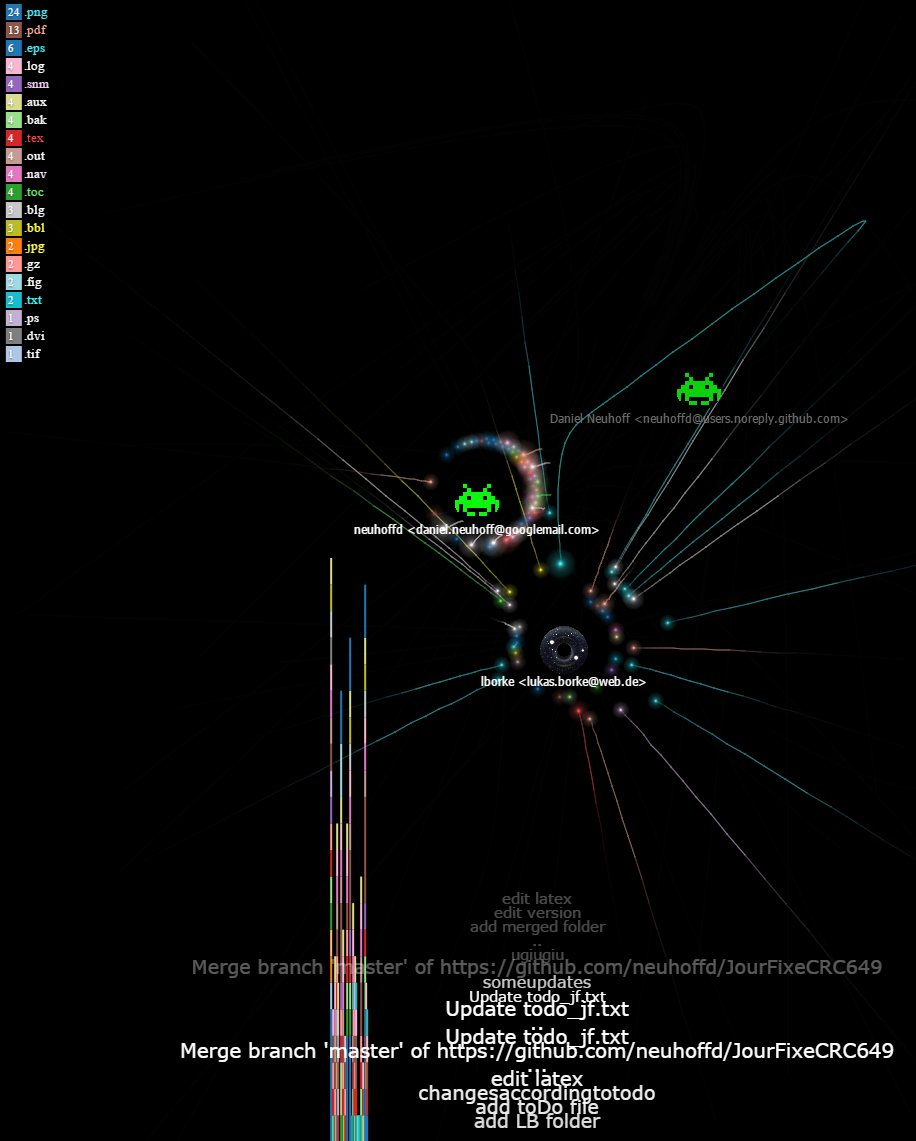
\includegraphics[scale=0.16]{colla_visu2}
				\vspace{-0.25cm}
				\caption{Snapshots of the 
					\href{https://github.com/neuhoffd/JourFixeCRC649}
					{development of this presentation}}
		\end{center}
		\end{figure}
		
		\vspace{-0.45cm}
		\begin{center}
		%\href{https://github.com/QuantLet/Git2Q3-Collaboration/blob/master/README.md}{Development of this presentation}
		\href{https://github.com/QuantLet/Git2Q3-Collaboration/blob/master/README.md}{More examples of collaboration projects}
		
		\end{center}
}



%%%%%%%%%%%%%%%%%%%%%%%%%%%%%%%%%%%%%%%%%%%%%%%%%%%%%%%%%%%%%%%%%%%%%%%%%%%%%%%%%%%%%%%%%%%%%%%%%%%%%%%%%%%%%%%%%%%%%%%%
\frame{
 	\begin{center}
		\textbf{Thank you for your attention!} 	
 	\end{center}
}

\end{document}

